%!TeX ts-program = xelatex
%!TeX encoding = utf-8 Unicode
\documentclass[ieeetran]{article}
\usepackage{amsmath, amssymb}
\usepackage{graphicx}

\title{Software Engineering for Business Applications Lecture Notes}
\author{Efe Kamasoglu}

\begin{document}

\maketitle

\pagebreak

\section{IT Support for Business Applications} % (fold)
\label{sec:iT_support_for_business_applications}

\subsection{Classification of Business Applications} % (fold)
\label{sub:classification_of_business_applications}

\begin{itemize}
  \item \textbf{Definition "Business Application":}
	  \begin{itemize}
	    \item \underline{in narrower sense:} totality of all programs, i.e.\ \textbf{application software}, and associated \textbf{data} for a concrete business use case
	    \item \underline{in broader sense:} additionally \textbf{hardware}, \textbf{system software} and necessary \textbf{communication} facilities required for the use of application software
	  \end{itemize}
\item \textbf{Two roles of Business Applications:}
	\begin{itemize}
	  \item \textbf{supporting}, \textbf{improving} or \textbf{automating} existing operational processes in bookeeping, accounting, etc.\ (size, speed, correctness...)
	\item \textbf{enabling} new products and services (e.g.\ online shopping and banking)
	\end{itemize}
\item \textbf{Classification of Business Applications by Business Purpose:}
	\begin{figure}[h!]
	  \centering
	  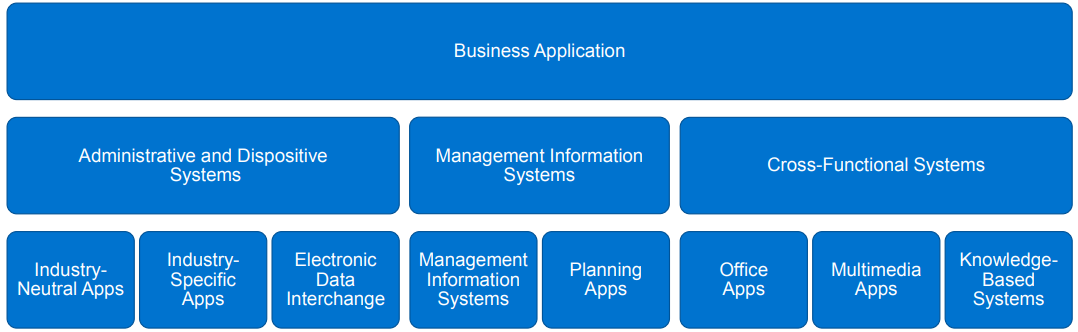
\includegraphics[width=0.5\linewidth]{classofba.png}
	  \label{fig:classofba_png}
	\end{figure}

\textit{\underline{Examples of}}

\begin{itemize}
  \item \textbf{administrative systems:} financial accounting, payroll accounting, administration of stocks
\item \textbf{disposition systems:}\ calculation and cost accounting, material procurement, field service control
\item \textbf{management information systems (MIS):} use of internal company data, use of external data, combination of multiple data sources in a flexible form
\item \textbf{planning systems:}\ planning of individual functional areas, integrated planning of several functional areas, corporate planning

\end{itemize}
\item \textbf{Cross-Cutting Applications:}
	\begin{itemize}
	  \item independent of compant hierarchy and fuctional domains
	\item used either directly via user interface or programmatically via administration and disposition systems
	\item \textit{Examples:} office suites, groupware, workflow management systems
	\end{itemize}

\item \textbf{Enterprise Resource Planning (ERP):} \textbf{ERP system} is an integrated business application (suite, collection of programs), which supports all essential functions of administration, disposition and management with a \underline{common interface and a shared and integrated data management}.
	\begin{itemize}
	  \item consists of platform and function-oriented application components that exchange info and events
          \item is realized as (customizable) standard software
	\item \textit{Examples:} external accounting, controlling, procurement
	\item Today's ERP systems support an \textbf{extended value chain}\footnote{\textbf{Value chain} is a business model that describes the full range of activities needed to create a product or service.}.
	\end{itemize}
\end{itemize}

\subsection{Standard and Custom Software} % (fold)
\label{sub:standard_and_custom_software}

\begin{itemize}
  \item \textbf{Standard Software vs. Custom Software:}
	  \begin{itemize}
	    \item \textbf{Standard software}\textit{(e.g.\ SAP)}
		    \begin{itemize}
		      \item developed for specific \textbf{market}
		\item distributed by a software house
			\item can be used by \textbf{several companies}
			\item implements "standard business processes" at its core
			\item maintained by \textbf{manufacturer}, adapted to changes
			\item must or can be \textbf{customized} to company (e.g.\ authorizations and roles, currencies) 
		    \end{itemize}
	\item \textbf{Custom software}
		\begin{itemize}
		  \item specifically developed for \textbf{one company}
	\item tailored to specific business processes/requirements
		\item result of a project for a known client
			\item \textbf{individually} maintained and adapted to changes
		\end{itemize}
	  \end{itemize}
\pagebreak
\item \textbf{Adaptation Techniques for Standard Business Software:}
	\begin{itemize}
		\item Adaptation of operational standard software can be divided into \textbf{Configuration}, \textbf{Extension} and \textbf{Coupling} (= \textbf{Customizing}).
               \begin{figure}[h!]
                 \centering
                 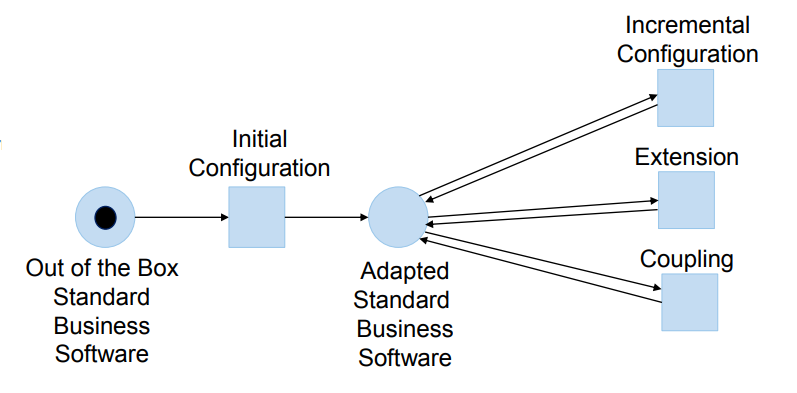
\includegraphics[width=0.5\linewidth]{adaptationsbs.png}
                 \label{fig:adaptationsbs_png}
               \end{figure} 

	       \item \textbf{Configuration} describes functionalities and techniques
		       \begin{itemize}
		         \item that are obligatory on first deployment
				 \item that allow to define predefined settings
			\item that lead to an individual variation of standard software
		       \end{itemize}

	\item \textbf{Extension} describes functionalities and techniques
		\begin{itemize}
		  \item that are optional for productive use
			  \item that allow to map requirements not foreseen by manufacturer
				  \item implemented by manufacturer to expand the range of services
		\end{itemize}

		\item \textbf{Coupling} refers to functionalities and techniques
			\begin{itemize}
			  \item to connect external systems of other manufacturers
				  \item to connect external systems of the same type
				\item that are predefined in the form of data file formats, APIs, or communication protocols
			\end{itemize}


		\item \textit{Example:} mapping the structure of a company to SAP applications via organizational units (can be assigned to single or multiple apps)
	\end{itemize}

	\item \textbf{Configuration: Challenges}
		\begin{itemize}
		  \item A \textbf{standard software} must
			  \begin{itemize}
			    \item provide all relevant configuration options
			\item support a wide range of different corporate structures and processes
			\item check dependencies between these many variants
			\item provide appropriate documentation about the effects of individual configurations

			  \end{itemize}
		  \item \textbf{Consequences:} 
				  \begin{itemize}
				    \item need for experts who are familier with configuration options of each release and componant
					   \item scarcity of such experts
						   \item expensive training
							   \item expensive consultancy services
				  \end{itemize}
		\end{itemize}

\item \textbf{Examples for Extensions:}
	\begin{itemize}
	  \item automation of \textbf{multi-step business workflows}
	\item integration of company-specific calculations/rules/checks
	\item connecting customers
	\end{itemize}
\item \textbf{Coupling Options:}
	\begin{itemize}
	  \item different coupling options depending on the scenario
	\item programming language used for coupling
	\item available mechanisms to couple
	\end{itemize}

\item \textbf{Multi Tenancy:} Software multitenancy is a software architecture in which a single instance of software runs on a server and serves multiple tenants (e.g.\ companies).
	\begin{itemize}
	  \item sevearal companies can be represented in one system
	\item distinction between tenant-dependent and -independent data
	\item supporting tenant-dependent authorization (e.g.\ A may only perform transactions in client 002)
         \item individual adaptations of tenants (e.g.\ currency, couplings)
	\end{itemize}

\item \textbf{Multilingualism:}

	\begin{itemize}
	\item \textbf{Multilingualism of a business information system} makes it possible to
		\begin{itemize}
		  \item store and display texts in different languages in the system
		\item assing graphics and symbols specific to different languages 
		\end{itemize}
	
\item Multilingualism requires
	\begin{itemize}

\item that one system can process all relevant character sets at once
	\item storage and recognition of words, numbers etc.
	\item that a system can assign users to languages or user can choose their own
	\item that texts (graphics, symbols) can be assigned to a language
	\end{itemize}
	\end{itemize}
\item \textbf{Localization (l10n):} Adaptation of a software product to meet the language, culture, and other requirements of each locale (e.g.\ adaptation of graphics, currencies, date and time)
\item \textbf{Internationalization (i18n):}\ Process of preparing a software-based product for localization (to support global markets)
\end{itemize}

\subsection{Characteristics of Business Applications} % (fold)
\label{sub:characteristics_of_business_applications}
\begin{itemize}
  \item \textbf{Multiple Stakeholders and changing requirements:}
	  \begin{itemize}
	    \item \textbf{Requirements Elicitation and Requirements Management}
		    \begin{itemize}
		      \item many stakeholders, different views and concerns
		\item Waterfall: upfront requirements document and/or technical specification => Req. Documentation
		\item Issue: changing requirements once IT support is implemented
		\item Agile: incremental and iterative => Agile Req. Engineering
			\item typically, very large number of requirements
			\item need for formalization and early consistency checking => Conceptual Modeling
				\item need for cost and time prediction => Software Estimation

		    \end{itemize}

	\item \textbf{Programming Challenges}
		\begin{itemize}
		  \item design, implement and test changes in an existing complex system => Change Mgmt.
	\item deliver incremental changes without invalidating existing data => Release Mgmt.
		\item parallel development at manufacturer and at customer site => Version Mgmt.

		\item automated and quality-controlled assembly of application software => Build Mgmt.
		\end{itemize}
	  \end{itemize}

\item \textbf{Persistent Data and Concurrent Data Modification:}
	\begin{itemize}
	  \item \textbf{Data consistency} is a must:
		  \begin{itemize}
		    \item many users perform \textbf{transactions} simultaneously on central databases
		\item data must not be lost even in case of system failures.
		  \end{itemize}
		  \item \textbf{Programming challenges:}
			  \begin{itemize}
			    \item database is managed by an independent application, on a different server / hardware
			\item object orientation is not supported by common data bases
				\item database concepts must be transferred to the application logic (transactions, rights, primary keys)
			  \end{itemize}
	\end{itemize}

\item \textbf{Distributed Actors and Data Repositories:}
	\begin{itemize}
	  \item \textbf{Many users access central data concurrently:}
		  \begin{itemize}
		    \item users need data in different locations at different times
			    \item Client-Server architecture => Layered Architectures
		\item web clients => REST protocol
		  \end{itemize}

	\item \textbf{Programming challenges:}
		\begin{itemize}
		  \item software components must be able to found in network => Naming services
		  \item communication always via a network => Serialization\footnote{\textbf{Serialization} is the process of translating a data structure into a format that can be stored or transmitted and reconstructed later.} \& failed execution
			  \item authentication and authorization => Security
		\item concurrent accesses => Transactions
		\end{itemize}
	\end{itemize}

\item \textbf{Integeration of Data and Application from (Semi-)Autonomous Sources:}
	\begin{itemize}
	  \item \textbf{Separation of applications and data repositories:}
		  \begin{itemize}
		    \item multiple apps work on independent or shared data resources
			    \item multiple apps communicate with each other => RPC, Message Passing
			\item business processes involve multiple apps => Workflow Mgmt. Systems
			\item application landscapes with lots of interacting applications => Enterprise Architecture Mgmt.
		  \end{itemize}

		  \item \textbf{Programming challenges:}
			  \begin{itemize}
				  \item integration of multiple languages and databases
				\item loose coupling through interfaces to avoid code change propagationi
				\item error recovery to avoid runtime failure propagation
			  \end{itemize}
	\end{itemize}

\item \textbf{Scalability:}
	\begin{itemize}
	  \item \textbf{Growing number of users and data volume}
		  \begin{itemize}
		    \item business apps are used by thousands of employees world-wide around the clock
		\item customers and business partners interact directly with business apps and expect real-time sub-second response times
		\item volatile load (e.g.\ online shop in christmas season vs.\ summer season)
		  \end{itemize}
		  \item \textbf{Programming challenges:}
			  \begin{itemize}
				  \item delayed execution of resource-intesive operations => Batch processing\footnote{\textbf{Batch processing} is when a computer processes a number of tasks that it has collected in a group. It is designed to be a completely automated process, without human intervention.}
				    \item dynamically increasing/decreasing number of users => Instance pools
					    \item single server cannot handle the load => Load balancing, Caching
		
			  \end{itemize}
	\end{itemize}
\end{itemize}

\section{Requirements Engineering} % (fold)
\label{sec:requirements_engineering}

\begin{itemize}
  \item \textbf{Requirements engineering} is concerned with \textbf{elicitation}, \textbf{analysis}, \textbf{specification} and \textbf{validtion} of software requirements as well as the management of requirements.

\item \textbf{Software requirements} express the needs and constraints placed on a software product.
\end{itemize}

\subsection{Traditional Requirements Engineering} % (fold)
\label{sub:traditional_requirements_engineering}



% subsection traditional_requirements_engineering (end)





















% section requirements_engineering (end)
% subsection characteristics_of_business_applications (end)

% subsection standard_and_custom_software ()

% subsection classification_of_business_applications (end)

% subsection business_without_iT_support (end)

% section iT_support_for_business_applications (end)



\end{document}
